\chapter{EXPERIMENTAL SETUP AND DATA}
\label{chp:exp-setup-data}
The data used throuhout this thesis is taken from the database belonging Boğaziçi University Lung Acoustics Laboratory. All sound and airflow samples were recorded with the device developed in this laboratory. (İpek Sen Masters) The recording device has 14 channels. Each channel has the same analog interface, which includes a Sony ECM-44 BPT electret microphone followed by an analog amplifier with gain 100 which has a instrumentation amplifier based design. The amplification unit is followed by a $6^{th}$ order Butterworth low pass filter which have 4000 Hz cut-off and a $8^{th}$ order Bessel high pass filter whose cutoff is 80 Hz. The airflow recordings was done with a Validyne CD379 pneumatachograph. The digitization unit is the National Instrument's DAQCard-6024E which is operating at 9600 Hz and has 12 bit resolution. Each recording has a duration of 15 seconds \cite{ipek-device}.
\paragraph{} There are 23 healthy subjects in this study. The sounds were recorded at 14 different locations on chest wall. Locations of channels are shown in \ref{fig:mic_loc}.
\begin{figure}
	\begin{center}
		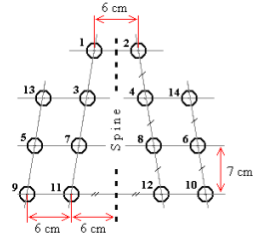
\includegraphics[width=0.4\textwidth]{figures/mic_loc.png}
		\caption{Microphone Locations on the Chest Wall \cite{ipek-phd-2}}
		\label{fig:mic_loc}
	\end{center}
\end{figure} \par